\documentclass{article}
\usepackage{amsmath}
\usepackage{graphicx}
\usepackage{datetime}
\usepackage{geometry}
\usepackage{placeins}
\usepackage{minted}
\usepackage{xcolor}
\usepackage{caption}
\usepackage{lmodern} 
\usepackage[document]{ragged2e}
\usepackage[hidelinks]{hyperref}
\usepackage{enumitem}
\geometry{
 a4paper,
 left=25mm,
 top=25mm,
 }
\captionsetup{hypcap=false} 
\newdateformat{daymonthyear}{\THEDAY .\THEMONTH .\THEYEAR}
\title{
  \centering
  
\includegraphics[width=\textwidth]{images/logo_PWr_kolor_poziom.png}\\
  \fontsize{28pt}{30pt}\selectfont Sprawozdanie 6\\
  \fontsize{14pt}{30pt}\selectfont Ćwiczenie 6.Akwizycja danych \linebreak DHT11 z wykorzystaniem łączności WiFi}
\author{Krzysztof Zalewa,Wiktor Wojnar}
\date{\daymonthyear\today}
\renewcommand*\contentsname{Spis treści}
\renewcommand{\figurename}{Rysunek}
\renewcommand{\listingscaption}{Fragment kodu}
\begin{document}
    \maketitle
    \pagebreak
    \tableofcontents
    \FloatBarrier
    \section{Wstęp teoretyczny}
        \subsection{Charakterystyka i zasady działania systemu FreeRTOS}
            FreeRTOS jest systemem operacyjnym czasu rzeczywistego (ang. Real time operating
            system) dla systemów wbudowanych. FreeRTOS został zaprojektowany tak by kod 
            źródłowy był prosty i krótki. Takie podejście pozwala na użycie go nawet na 
            najmniejszych urządzeniach. 
        \subsection{Wątki w FreeRTOS}
            \begin{figure}[ht]
                \centering
                \includegraphics[width=\textwidth]{images/Screenshot 2025-01-13 at 13-40-25 RTOS Fundamentals - FreeRTOS™.png}
                \caption{Wykonywanie wielu zadań[2]}
                \label{fig:multithread}
            \end{figure}
            \FloatBarrier
            W systemach takich jak Linux programy wykonywalne implementowane są przez jeden
            lub więcej wątków. W systemach RTOS wątki zwykle nazywane są zadaniami. Jedno
            rdzeniowe processory mogą wykonywać tylko jedną operacje w danym momencie. 
            Jednakże poprzez szybkie przełączanie między wykonywanym zadaniem można zbliżyć
            się do wykonywania wielu zadań jednocześnie. Za wybór które zadanie powinno być
            wykonywane odpowiada planista (ang. scheduler).
        \subsection{DHT11}
            \begin{figure}[ht]
                \centering
                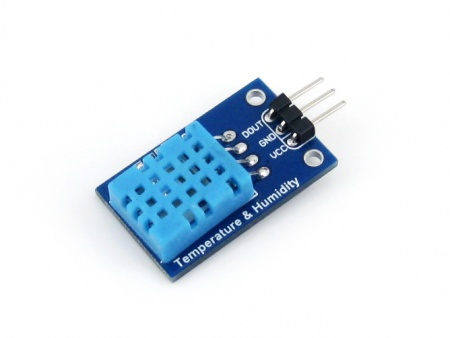
\includegraphics[width=\textwidth]{images/450px-Temperature-Humidity-Sensor_l.jpg}
                \caption{Płytka DHT11[3]}
                \label{fig:DHT11}
            \end{figure}
            \FloatBarrier
            \subsubsection{Budowa}
                DHT11 zawiera w sobie cyfrowy sensor temperatury i wilgoci. Według \hyperref[src:datasheet]{źródła~\ref*{src:datasheet}}
                układ ten do pomiaru temperatury wykorzystuje układ NTC a do pomiaru wilgotności
                układ oporowy. Wykonywane pomiary są w zakresie:
                \begin{enumerate}
                    \item Temperatura 0-50\(^\circ\text{C}\) błąd \(\pm 2^\circ\text{C}\)
                    \item Wilgotność 20-90\% RH \(\pm 5\%\text{ RH}\)
                \end{enumerate}
            \subsubsection{Zasady działania}
                \raggedright
                Pomiar wilgotności polega na pomiarze zmiany rezystancji w materiale pomiarowym.
                Jako że rezystancja zależy też od temperatury materiale to do urządzenia musi być
                dołączony układ pomiaru temperatury.\linebreak
                Pomiar temperatury tak samo jak w przypadku wilgotności polega na pomiarze
                rezystancji. Do wykonania takiego pomiaru używa się termistora (rezystora o 
                rezystancji silnie zależnej od temperatury). Rezystor NTC ma ujemny współczynnik 
                temperturowy (wzrost temperatury powoduje zmniejszenie rezystancji)
                \begin{figure}[ht]
                    \centering
                    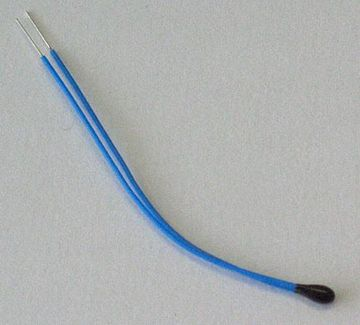
\includegraphics[width=\textwidth]{images/360px-NTC_bead.jpg}
                    \caption{Termistor NTC}
                    \label{fig:NTC}
                \end{figure}
                \FloatBarrier
    \section{Zadanie laboratoryjne}
        \subsection{Treść zadania}
            W ramach zadania laboratoryjnego należało skonfigurować układ ESP32 i uruchomić przykładowy 
            program. Następnie należało zainstalować system FreeRTOS oraz uruchomić wątki (1-akwizycji 
            pomiarów, 2-przetwarzania danych, 3-transmisji wyników). Na koniec należało rozbudować 
            wątki 1 i 2 w stopniu uzgodnionym z prowadzącym. 
        \subsection{Opis działania programu}
            Zgodnie z zadaniem zaimplementowany program ma trzy główne wątki. Jeden do obsługi 
            łączności WiFi. Drugi do pobierania danych podłączonego z DHT11. Trzeci do wysyłania
            danych do użądzeń końcowych. W wyniku działania programu otrzymano prostą stronę
            HTML która zawiera napis : Temperature today is: X °C, and the humidity in the air is: Y.
            Gdzie X to temperatura pobrana z DHT11 a Y to wilgotność pobrana z DHT11.
        \subsection{Schemat połączenia}
            \begin{figure}[ht]
                \centering
                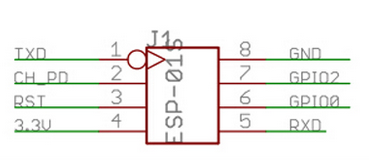
\includegraphics[width=\textwidth]{images/Zrzut ekranu 2025-01-27 004040.png}
                \caption{Schemat połączeń w płytce DHT11}
                \label{fig:DHT11schema}
            \end{figure}
            \FloatBarrier
            \begin{figure}[ht]
                \centering
                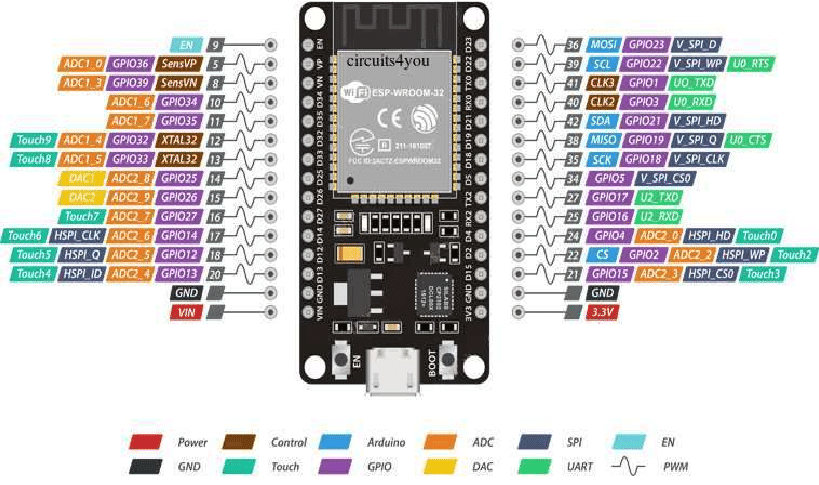
\includegraphics[width=\textwidth]{images/Pinout-diagram-of-ESP32.png}
                \caption{Schemat połączeń w płytce ESP32}
                \label{fig:ESP32schema}
            \end{figure}
            \FloatBarrier
            \begin{figure}[ht]
                \centering
                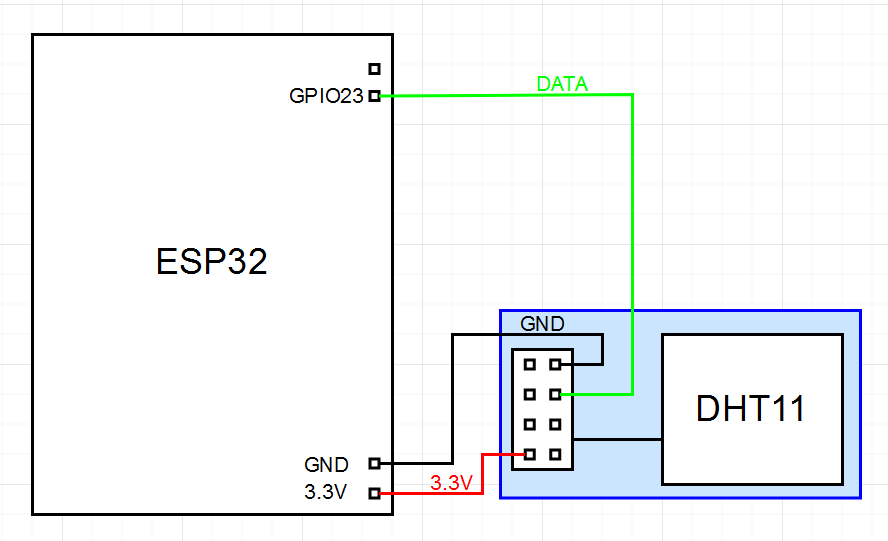
\includegraphics[width=\textwidth]{images/Zrzut ekranu 2025-01-27 003805.png}
                \caption{Schemat połączenia}
                \label{fig:schema}
            \end{figure}
            \FloatBarrier
            Płytka ESP32 była podłączona do płytki lutowanej w taki sposób że jedynie połowa portów
            była dostępna do użytku.Wybrane wejście GPIO23(General purpose input output) nie powinno 
            wpływać na funkcjonowanie programu.
        \subsection{Kod programu}
            \begin{frame}
                \scriptsize
                \inputminted[
                    style={vs},
                    breaklines,
                    breakanywhere, 
                    linenos, 
                    tabsize=4 
                ]{c++}{Lab6.cpp}
                \vspace{1em}
                \captionof{listing}{Fragment kodu z programu}
                \label{lst:code}
            \end{frame}
    \section{Źródła}
        \begin{enumerate}[label=\arabic*.]
            \item \url{http://www.embeddeddev.pl/kurs-freertos-wprowadzenie/}
            \item \url{https://www.freertos.org/Documentation/01-FreeRTOS-quick-start/01-Beginners-guide/01-RTOS-fundamentals}
            \item \url{https://www.waveshare.com/wiki/DHT11_Temperature-Humidity_Sensor}
            \item \url{http://wiki.sunfounder.cc/images/c/c7/DHT11_datasheet.pdf} \label{src:datasheet}
            \item \url{https://en.wikipedia.org/wiki/Hygrometer}
            \item \url{https://pl.wikipedia.org/wiki/Termistor}
        \end{enumerate}
\end{document}